\documentclass{article}
\usepackage{indentfirst}
\usepackage{amsmath}
\usepackage{amsfonts}
\usepackage{algpseudocode}
\usepackage{algorithm}
\usepackage{vmargin}
\usepackage{multirow}
\usepackage{graphicx}
\providecommand{\abs}[1]{\lvert#1\rvert}
\setpapersize{A4}

\title{\textbf{Silly Season Algorithm. Diseño e implementación de una metaheurística original}}
\author{Antonio José Blánquez Pérez}
\date{Práctica final Metaheurísticas - Universidad de Granada}

\begin{document}
	\setlength{\parskip}{1em}
	\maketitle
	
	\section{Proposición}
	\subsection{Motivación}
	\indent El concepto de esta metaheurística nace cuando, en medio de la cuarentena, la temporada 2020 de Formula 1 se está desarrollando de manera anómala. Esta comenzará en julio y no en marzo como es habitual\footnote{https://www.formula1.com/en/latest/article.f1-schedule-2020-latest-information.3P0b3hJYdFDm9xFieAYqCS.html}, provocando que la temporada dure hasta noviembre ininterrumpidamente también durante el mes de agosto(lo que nos dejará ver un Gran Premio de España el 16 de agosto, que se correrá a una temperatura poco convencional), se cancela el Gran Premio de Mónaco por primera vez desde 1955 y, lo que nos ocupa en este caso, debido al cambio en el calendario y a que en este deporte no existe un mercado de fichajes con fechas establecidas como, por ejemplo, en el fútbol, los equipos están dedicando su tiempo a cerrar fichajes para 2021, año en el que la mayoría de pilotos acaba contrato al ser fecha de cambio en el reglamento(aunque se ha retrasado a 2022). El término $Silly\ Season$, que da nombre a la metaheurística, se acuñó para definir el tiempo, generalmente los meses de verano, en el que a falta de noticias los medios de comunicación comienzan a hablar sobre rumores y, en el contexto del deporte, rumores sobre fichajes; aunque este término es ampliamente usado para referirse al período de fichajes que suele darse en los parones de verano e invierno. Aunque en el momento en el que se escriben estas líneas aún no es verano y deberíamos de estar a la espera del GP de Francia, la realidad es que esta temporada aún no ha comenzado y se ha desarrollado una Silly Season como no se recuerda en años\footnote{https://www.motorpasion.com/formula1/cascada-fichajes-formula-1-daniel-ricciardo-confirmado-como-sustituto-carlos-sainz-mclaren}.
	\par
	De esta situación surgió la idea de plantear una metaheurística basada en la ya comentada Silly Season, donde los pilotos serán individuos soluciones al problema que se organizarán en equipos o conjuntos que determinarán el trato que se le dará a cada individuo.
	
	\subsection{Resumen en contexto}
	\indent El funcionamiento de esta metaheurística se basa en unos elementos bien definidos, las soluciones, que serán nuestros pilotos, se generarán y organizarán en equipos inicialmente de manera aleatoria, y se les asignará una puntuación a través de la función objetivo. Los equipos cuyos pilotos tengan mejor puntuación serán los que estén en la zona alta de la tabla y viceversa. Como los equipos de la parte alta tienen más dinero no pueden arriesgarse a cambios relevantes en su organización, por lo que generalmente se centrarán en mejorar al máximo el rendimiento de su coche(y por tanto el de su piloto). Por otra parte los equipos de la parte, puesto que no tienen nada que perder, tienden a realizar grandes cambios tanto en su organización como en su plantilla. Es decir, en los equipos con mayor puntuación los pilotos evolucionarán mediante explotación y los que tengan una puntuación más baja lo harán mediante exploración. Además, tras un cierto período(la temporada o época) los pilotos cambiarán de equipo , aunque también habrá una posibilidad de que lo hagan entre temporadas.
	\par
	Este concepto se puede plantear como una buena metaheurística en la medida en la que se consigue equilibrar la exploración y la explotación controlando cuantas iteraciones hacen cada una en proporción, equilibrio que podría proporcionar una buena solución. Esto es porque intentaremos conseguir que las soluciones sean buenas mediante explotación en el caso de las que sean ya buenas en los que hemos definido como los mejores equipos y evitaremos óptimos locales mediante la exploración en el entorno de los peores equipos, ya que con ellos terminaremos consiguiendo soluciones potencialmente buenas.
	
	\section {Descripción detallada}
	\subsection{Concepto}
	En este apartado se va a concretar el funcionamiento comentado en la sección anterior, apoyándose en el pseudocódigo de abajo.\par
	\begin{algorithm}
	\caption{Silly Season Algorithm}\label{sillyseason}
	\begin{algorithmic}[1]
	\Procedure{Silly Season}{$dataset,constraints,k$}
		\For{$number\ of\ teams$}\Comment{Generate initial random solutions}
			\For{$number\ of\ pilots\ per\ team$}
				\State{$team.add(random\_solution)$}
			\EndFor
			\State{$teams.add(team)$}
		\EndFor
		\State $generate\ hierarchy\ vector$\Comment{Where $i$ value is the mean of $f$ values of team $i$}
		\While{$eval \le max\_eval$}
			\ForAll{team}
				\If{$hierarchy[team] > f\_mean$}\Comment{Where $f\_mean$ is the f mean of all pilots}
					\ForAll{$pilot$}
						\State $LS(pilot,BL\_max)$\Comment{Local Search with $BL\_max$ maximum evaluations}
					\EndFor
				\Else
					\ForAll{$pilot$}
						\State $mutate(pilot,mutation\_prob)$\Comment{Mutation with $mutation\_prob$ probability}
					\EndFor
				\EndIf
			\EndFor
			\If{$current\ season\ has\ finished$}
				\State $swap\ N\ pilots$
			\Else
				\State $swap\ M\ pilots$
			\EndIf
			\State $fix\ hierarchy$
		\EndWhile
		\State \textbf{return} $best\ solution$
	\EndProcedure
	\end{algorithmic}
	\end{algorithm}
	\newpage
	Primero el algoritmo genera un conjunto de soluciones aleatorias de manera que formarán conjuntos, los equipos, que tendrán cada uno un número de soluciones, los pilotos, determinado. El número de equipos y el de pilotos por equipo serán dos parámetros a tener en cuenta en la solución.
	\par
	A partir de los equipos podemos formar un vector de jerarquía con la media para cada equipo de los valores dados por la función de coste a los pilotos. Entonces se les aplicará Búsqueda Local a los pilotos de los equipos que superen la media, los equipos grandes, y se mutará a los que pertenezcan a los equipos que tengan peor media, los equipos pequeños. Las evaluaciones máximas para BL y la probabilidad de mutación habrán de tenerse también en cuenta.
	\par
	Esto se hará en bucle y, para cada iteración, si se ha terminado la temporada se intercambiarán de equipo $N$ parejas de pilotos aleatoriamente, si no ha terminado lo harán $M$ parejas, siendo generalmente $M<N$. Por supuesto es necesario ajustar la jerarquía tras el intercambio.
	\par
	Al superar el número máximo de evaluaciones el algoritmo devolverá la mejor solución encontrada hasta el momento.
	
	\subsection{Parámetros}
	Del concepto final del algoritmo aparecen varios parámetros que han de usarse para controlar el equilibrio entre exploración y explotación, en concreto 8:
	\begin{itemize}
		\item Número de equipos: variar este parámetro resultará importante en gran medida para determinar el tamaño de la población y, por tanto, el tiempo de ejecución.
		\item Número de pilotos por equipo: exactamente igual al anterior, ya que nuestra población final será el resultado de $n\_equipos\cdot n\_pilotos\_por\_equipo$.
		\item Número máximo de evaluaciones para BL: este parámetro será primordial para determinar el número de evaluaciones que hará BL por iteración, lo que resulta importante para el equilibrio explotación-exploración.
		\item Probabilidad de mutación: el caso opuesto al anterior para el equilibrio explotación-exploración. A mayor probabilidad más exploración existirá en proporción a la explotación.
		\item Número de intercambios entre temporadas: determinará el número de intercambios durante la Silly Season, importante para la explotación.
		\item Número de intercambios(por iteración) durante la temporada: mismo caso que el anterior para intercambios cuando una iteración no sea final de temporada.
		\item Máximo número total de evaluaciones: Como en todas las metaheurísticas, para poder tener una referencia de su bondad respecto a otras.
	\end{itemize}
	
	\section{Aplicación}
	\subsection{Descripción del problema}
	\indent El agrupamiento o clustering busca clasificar objetos de un conjunto en subconjuntos o clusters a
	través de sus posibles similaridades. Es una técnica de aprendizaje no supervisado que permite
	descubrir grupos inicialmente desconocidos o agrupar objetos similares, de manera que podemos
	encontrar patrones en grandes grupos de datos que serían imposibles(o extremadamente difíciles) de
	encontrar sin esta técnica.
	\par
	Un ejemplo cotidiano del problema del agrupamiento sería dividir una cantidad de frutas en verdes,
	poco maduras y muy maduras que, aunque trivial, nos permite entender el concepto que hay detrás
	de la técnica que nos ocupa. Con ésto podemos comprender otras aplicaciones del clustering, como
	pueden ser el análisis de caracteres escritos a mano, muestras de diálogo, huellas dactilares o
	imágenes, la clasificación de especies en subespecies o el agrupamiento para moléculas o proteínas.
	Para poder aplicar esta técnica debemos medir $d$ características de nuestro grupo de $n$ objetos, por
	ejemplo el color o la textura en el caso de las frutas o la simetría o la intensidad en el caso de
	caracteres escritos a mano, obteniendo una conjunto de datos de longitud $n$ con $d$ dimensiones.
	\par
	En nuestro caso concreto abordaremos una variación del clustering clásico, el Problema de
	Agrupamiento con Restricciones(PAR), es decir, además de nuestro conjunto de datos tenemos
	cierta información a la que llamaremos restricciones o, más concretamente, restricciones de
	instancia. Ésto quiere decir que tenemos alguna información sobre objetos que tienen que
	pertenecer al mismo cluster(ML, Must-Link) y sobre objetos que no pertenecen al mismo
	cluster(CL, Cannot-Link), siendo éstas restricciones débiles, o lo que es lo mismo, podemos
	incumplir restricciones pero debemos minimizar el número de incumplidas al máximo.
	El planteamiento combinatorio de este problema es NP-Completo, por tanto a continuación
	propondremos algunas alternativas de algoritmos para intentar resolver el problema de forma
	aproximada en un tiempo razonable. El problema se abordará con $k$(nº de clusters) conocida, ya que
	su búsqueda es otro problema complejo.
	
	\subsection{Formalización de conceptos del problema}
	Vamos a definir distintos conceptos que se nombrarán a lo largo del documento y que son
	necesarios para entender los procedimientos en cada algoritmo.
	Primeramente podemos formalizar la definición de nuestro conjunto de datos como una matriz $X$ de
	$n\cdot d$, $n$ objetos en un espacio de $d$ dimensiones(el número de medidas que tenemos sobre cada
	objeto).\par
	{\centering $\vec{x_i} =\{x_{i,1},...,x_{i,d}\}\ \vert \ x_{i,j}\in \mathbb R\ \forall j\in \{1,...,d\}$\par}
	Llamaremos $C=\{c_1,...,c_k\}$ al conjunto de los $k$ clusters, de manera que cada $c_i$ será un subconjunto
	de $X$ y podrá asociada una etiqueta $l_i$ que lo nombre Para cada cluster es posible calcular su
	centroide asociado $\vec{\mu_i} $ , siendo el vector promedio de sus instancias.\par
	{\centering $\vec{\mu_i} = \frac{1}{\abs{c_i}} \displaystyle\sum_{\vec{\mu_j} \in c_i} \vec{x_j}$\par}
	También debemos definir la distancia media intra-cluster, $c_i$ , como la media de las distancias
	entre cada instancia del cluster y su centroide asociado, usando en este caso la distancia euclídea,
	aunque es equivalente a usar, por ejemplo, la distancia Manhattan.\par
	{\centering ${\overline{c_i}} = \frac{1}{\abs{c_i}} \displaystyle\sum_{\vec{\mu_j} \in c_i} \abs{\abs{\vec{x_j}-\vec{\mu_i}}} $\par}
	A través de estas, podemos llegar a la desviación general de $C$, la media de las desviaciones intracluster,
	que nos será de gran ayuda para minimizar la solución y para su posterior análisis.\par
	{\centering ${\overline{C}} = \frac{1}{k} \displaystyle\sum_{c_i \in C} \overline{c_i}$\par}
	Por otro lado tenemos las restricciones, $R=ML\cup CL$, donde $ML(\vec{x_i},\vec{x_j})$ indica que las
	instancias $\vec{x_i}$ y $\vec{x_j}$ deben estar asignadas al mismo cluster y $CL(\vec{x_i},\vec{x_j})$ que las instancias
	$\vec{x_i}$ y $\vec{x_j}$ no pueden ser asignadas al mismo cluster. Con ello, definimos la infactibilidad o
	infeasibility, que es un indicador de las restricciones que incumple nuestra solución.\par
	{\centering $infeasibility=\displaystyle\sum_{i=0}^{\abs{ML}}1(h_c(\vec{ML}_{[i,1]})\neq h_c(\vec{ML}_{[i,2]}))+\displaystyle\sum_{i=0}^{\abs{CL}}1(h_c(\vec{CL}_{[i,1]})=h_c(\vec{CL}_{[i,2]}))$\par}
	Siendo 1 la función booleana que devolverá 1 si la expresión que toma como argumento es verdadera y 0 en otro caso.
	
	\subsection{Representación de la información}
	Ahora que tenemos algunos conceptos claros y formalizados, pasamos a ver como representaremos
	la información necesaria en el proceso de resolución del problema.
	Primero aclarar que los datos de entrada, nuestro conjunto de datos, estará organizado en una matriz
	implementada como un vector$<$vector$<$float$>>$ (ambos vectores de la librería STL), es decir, un
	vector de longitud $n$ de vectores de reales en coma flotante de longitud $d$.
	Para las restricciones usaremos dos formas de representación, una para facilitar el acceso cuando
	conocemos la restricción que queremos comprobar y otra para cuando queramos recorrer todas las
	restricciones. Para el primer caso se usará la misma representación que para el dataframe, mientras
	que para el segundo se construirá una lista con elementos del tipo $[x,y,{1,-1}]$, siendo $x$ e $y$ los dos
	elementos que tiene la restricción y el último elemento 1 si conforman una restricción ML y -1 si es
	CL. Esta lista se ha implementado usando un vector$<$vector$<$int$>>$, también de la STL. De ésta
	manera, al recorrer esa lista evadiremos todos los pares que no tienen una restricción y nuestra
	búsqueda será mucho más eficiente que en una matriz.
	Por último, representaremos la solución con un vector$<$int$>$ de longitud $n$, de manera que la
	posición $i$ contendrá el número del cluster asignado al objeto $i$.
	
	\subsection{Función objetivo}
	La función objetivo es la función que debemos minimizar, es decir, la función que dice como de
	buena es la solución que le pasamos como parámetro.
	De todas las definiciones que hemos hecho, desviación general($\overline{C}$) e infactibilidad(infeasibility)
	nos dan información acerca de la bondad de la solución, la primera a través de la distancia promedio
	de cada dato a su centroide correspondiente y la segunda a través de la medida del incumplimiento
	de las restricciones de la solución dada. Ambas han de ser minimizadas, pero hay que darle más o
	menos importancia a una y a otra, de manera que debemos introducir un parámetro con el que
	controlar ésta importancia que debatiremos posteriormente.\par
	{\centering $f = \overline{C}+infeasibility\cdot \lambda$\par}
	Dicho ésto queda definir el parámetro $\lambda$, el cual se ha decidido proponer como el entero superior a
	la distancia máxima $D$ dividida por el número de restricciones totales $R$.\par
	{\centering $\lambda = \frac{\lceil D \rceil}{\abs{R}}$\par}
	
	\subsection{Conjuntos de datos usados}
	Los conjuntos de datos usados para testear la bondad de los algoritmos son los siguientes:
	\begin{itemize}
		\item Iris: Contiene información sobre las características de tres tipos de flores de Iris. Tiene 3
		clases(k=3) y 6 dimensiones.
		\item Ecoli: Contiene medidas sobre las ciertas características de diferentes tipos de células que
		pueden ser empleadas para predecir la localización de ciertas proteínas. Tiene 8 clases(k=8)
		y 7 dimesiones.
		\item Rand: Conjunto de datos artificial formado por tres agrupamientos bien diferenciados
		generados en base a distribuciones normales. Tiene 3 clases(k=3) y 2 dimensiones.
		\item Newthyroid: Contiene medidas cuantitativas tomadas sobre la glándula tiroides de 215
		pacientes. Tiene 3 clases(k=3) y 5 dimensiones.
	\end{itemize}
	
	\section{Manual de usuario}
	\textbf{Compilación:} Se incluye un makefile, por lo que se compila tan solo ejecutando la orden ‘make’ desde la terminal en la carpeta que contiene el código.\par
	\textbf{Ejecución:} Para ejecutar el algoritmo sobre un conjunto de datos concreto se hará mediante la siguiente orden en la terminal.\par
	{\centering ./silly\_season $<$fichero\_datos$>$ $<$fichero\_restricciones$>$ $<k>$ $<$seed$>$\par}
	También es posible llamarlo sin argumentos, entonces pedirá por teclado la información necesaria, o usar el script incluído, que replicará todos el experimento realizado para el análisis de rendimiento.
	
	\section{Análisis de rendimiento}
	\subsection{Descripción de los casos del problema}
	Se van utilizar todos los conjuntos de datos anteriormente mencionados para analizar como de buenos son los algoritmos planteados para resolver el problema del agrupamiento con restricciones, con el 10 y el 20\% de restricciones en cada conjunto de datos. Los datos se organizan en tablas y se analizarán posteriormente. Para ello se quería realizar con cada uno de los cuatro conjuntos, Iris, Newthyroid, Ecoli y Rand,
	tanto con el 10\% como con el 20\% de restricciones, un total de 5 veces, lo que hace un total de 40 ejecuciones(4 conjuntos x 2 conjuntos de restricciones x 5 veces). Sin embargo, como veremos, Ecoli resulta un problema en cuanto a tiempo de ejecución, por solo se ha podido obtener las soluciones con una semilla. Para poder replicar el total de ejecuciones todas ellas se han realizado utilizando semillas para la generación de números aleatorios, por lo que conociendo estas semillas se puede realizar el estudio exactamente de la misma manera y con los mismos resultados. Las semillas usadas en este estudio son las siguientes:\par
	{\centering
	\begin{tabular}{|c|c|c|c|c|}
		\hline
		Ejecución 1 & Ejecución 2 & Ejecución 3 & Ejecución 4 & Ejecución 5 \\
		\hline
		798245613 & 798245613 & 25022020 & 17042026 & 459268694 \\
		\hline
	\end{tabular}
	\par}
	\subsection{Resultados obtenidos}
	En las siguientes tablas se muestra el resultado de las pruebas anteriormente mencionadas a excepción de Ecoli, que como se verá requiere un tiempo de ejecución excesivamente alto y por tanto solo se ha realizado una ejecución para cada conjunto de restricciones, cuyo resultado es el que se añade a las últimas tablas para comparar datos. También es necesario recalcar que se han recogido los algoritmos más relevantes de cada práctica y que, tanto el algoritmo genético como el memético, no son los míos si no que son cedidos por Ángel de la Vega Jiménez para poder hacer la comparación ya que mi práctica 2 tiene varios problemas que no he tenido tiempo de solucionar y que no son objetivo de esta práctica.
	{\centering
	\begin{table}[]
		\resizebox{15cm}{!}{
		\begin{tabular}{lllllllllllll}
			\multirow{2}{*}{SSA 10\%} & \multicolumn{4}{l}{\textbf{Iris}}                                                             & \multicolumn{4}{l}{\textbf{Newthyroid}}                                                       & \multicolumn{4}{l}{\textbf{Rand}}                                                             \\
			& \textit{\textbf{Tasa\_C}} & \textit{\textbf{Tasa\_inf}} & \textit{\textbf{Agr.}} & \textbf{T} & \textit{\textbf{Tasa\_C}} & \textit{\textbf{Tasa\_inf}} & \textit{\textbf{Agr.}} & \textbf{T} & \textit{\textbf{Tasa\_C}} & \textit{\textbf{Tasa\_inf}} & \textit{\textbf{Agr.}} & \textbf{T} \\
			\textbf{Ej 1}      & 0,669                     & 0                           & 0,669                  & 12,219     & 10,82                     & 109                         & 12,64                  & 65,86      & 0,716                     & 0                           & 0,716                  & 16,719     \\
			\textbf{Ej 2}      & 0,669                     & 0                           & 0,669                  & 36,688     & 10,84                     & 109                         & 12,66                  & 125,83     & 0,716                     & 0                           & 0,716                  & 28,906     \\
			\textbf{Ej 3}      & 0,669                     & 0                           & 0,669                  & 16,484     & 10,88                     & 100                         & 12,55                  & 65,94      & 0,716                     & 0                           & 0,716                  & 18,969     \\
			\textbf{Ej 4}      & 0,669                     & 0                           & 0,669                  & 18,609     & 10,82                     & 109                         & 12,64                  & 99,11      & 0,716                     & 0                           & 0,716                  & 15,938     \\
			\textbf{Ej 5}      & 0,669                     & 0                           & 0,669                  & 14,594     & 10,88                     & 97                          & 12,50                  & 92,88      & 0,716                     & 0                           & 0,716                  & 19,250     \\
			\textbf{Media}            & 0,669                     & 0,0                         & 0,669                  & 19,719     & 10,847                    & 104,8                       & 12,597                 & 89,922     & 0,716                     & 0,0                         & 0,716                  & 19,956    
		\end{tabular}}
	\end{table}}

	{\centering
	\begin{table}[]
		\resizebox{15cm}{!}{
		\begin{tabular}{lllllllllllll}
			\multirow{2}{*}{SSA 20\%} & \multicolumn{4}{l}{\textbf{Iris}}                                                             & \multicolumn{4}{l}{\textbf{Newthyroid}}                                                       & \multicolumn{4}{l}{\textbf{Rand}}                                                             \\
			& \textit{\textbf{Tasa\_C}} & \textit{\textbf{Tasa\_inf}} & \textit{\textbf{Agr.}} & \textbf{T} & \textit{\textbf{Tasa\_C}} & \textit{\textbf{Tasa\_inf}} & \textit{\textbf{Agr.}} & \textbf{T} & \textit{\textbf{Tasa\_C}} & \textit{\textbf{Tasa\_inf}} & \textit{\textbf{Agr.}} & \textbf{T} \\
			\textbf{Ej 1}      & 0,669                     & 0                           & 0,669                  & 17,141     & 10,72                     & 309                         & 13,42                  & 59,78      & 0,716                     & 0                           & 0,716                  & 14,328     \\
			\textbf{Ej 2}      & 0,669                     & 0                           & 0,669                  & 32,297     & 13,55                     & 41                          & 13,91                  & 117,53     & 0,716                     & 0                           & 0,716                  & 10,406     \\
			\textbf{Ej 3}      & 0,669                     & 0                           & 0,669                  & 17,688     & 10,74                     & 329                         & 13,61                  & 73,94      & 0,716                     & 0                           & 0,716                  & 16,000     \\
			\textbf{Ej 4}      & 0,669                     & 0                           & 0,669                  & 13,109     & 10,83                     & 255                         & 13,05                  & 88,23      & 0,716                     & 0                           & 0,716                  & 14,422     \\
			\textbf{Ej 5}      & 0,669                     & 0                           & 0,669                  & 14,594     & 10,88                     & 293                         & 13,43                  & 79,98      & 0,716                     & 0                           & 0,716                  & 15,047     \\
			\textbf{Media}            & 0,669                     & 0,0                         & 0,669                  & 18,966     & 11,344                    & 245,4                       & 13,484                 & 83,894     & 0,716                     & 0,0                         & 0,716                  & 14,041    
		\end{tabular}}
	\end{table}}

	\begin{figure}[H]
		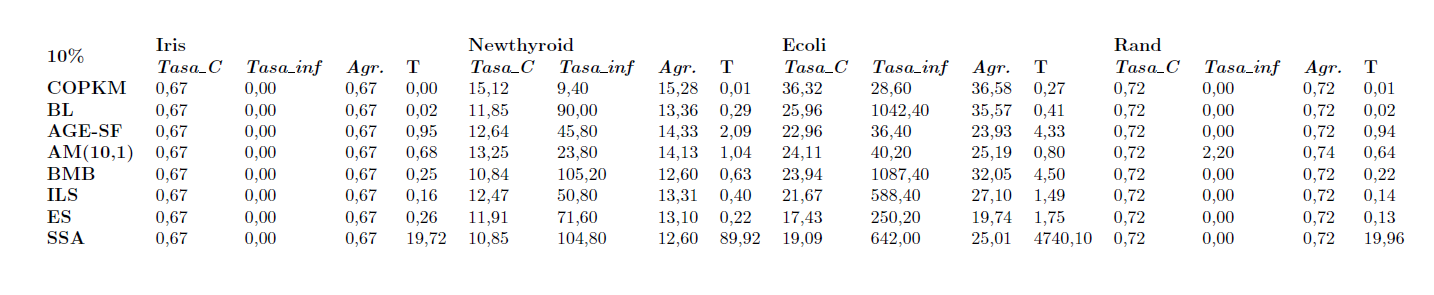
\includegraphics[width=\linewidth]{imagenes/tabla10.png}
		\label{fig:boat1}
	\end{figure}

	\begin{figure}[H]
		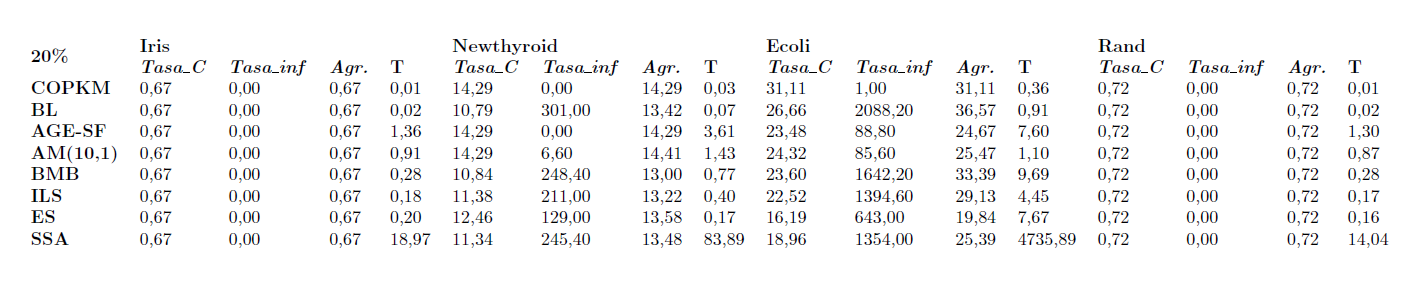
\includegraphics[width=\linewidth]{imagenes/tabla20.png}
		\label{fig:boat2}
	\end{figure}

	En cuanto a los parámetros se han decidido usar 5 equipos de 2 pilotos cada, con temporadas de 10000 evaluaciones en las que se hace 1 intercambio de pilotos a cada iteración durante la temporada y 4 cuando esta acaba. Las iteraciones máximas para BL se han establecido en 1000 y la probabilidad de mutación en una mutación por cada 1050 "genes"; siendo todos estos parámetros regulados en función de pruebas en las que se buscaba un buen equilibro explotación-exploración, objetivo de cualquier metaheurística. Para poder compararla con el resto de algoritmos se ha establecido el número máximo de evaluaciones en 100000.

	\subsection{Análisis de resultados}
	
	A partir de los resultados obtenidos podemos sacar varias conclusiones. La primera, que se puede ver en los gráficos de 10 y 20\% de restricciones, es que SSA(Silly Season Algorithm) es bastante competente, en concreto para Newthyroid encuentra soluciones muy cercanas a las mejores para el resto de algoritmos y para Ecoli(para las única prueba que ha podido realizarse), sorprendentemente solo es peor que Enfriamiento Simulado, AGE y Memético. No tiene sentido hablar de Iris y Rand ya que salvo algunas excepciones sin importancia para todos los casos se optiene el óptimo. Como ya se ha hablado en prácticas, a partir de los resultados obtenidos se puede deducir que en ese equilibrio explotación-exploración ya comentado Newthyroid obtiene mejores resultados fomentando la explotación, mientras que Ecoli suele funcionar mejor con un enfoque explorativa, aunque cuando realmente se consigue un buen resultado es con un equilibrio lo más óptimo posible como podemos ver en los resultados obtenidos por ES. A la vista de esto, vemos que SSA es capaz de obtener buenos resultados en ambos casos, acercándose aunque quedándose atrás de ES, que se perfila como el mejor algoritmo utilizado hasta el momento, y devolviendo mejores resultados que algoritmos ya buenos de por sí como ILS. También se puede ver una clara coincidencia con los Algoritmos Meméticos, lo cual es lógico ya que el funcionamiento es muy parecido con la salvedad de que en AM se aplican cruces y BL a toda la población, mientras que en SSA no se aplican cruces, solo mutaciones, y se usan ambas técnicas de manera disjunta.
	
	\begin{figure}[H]
		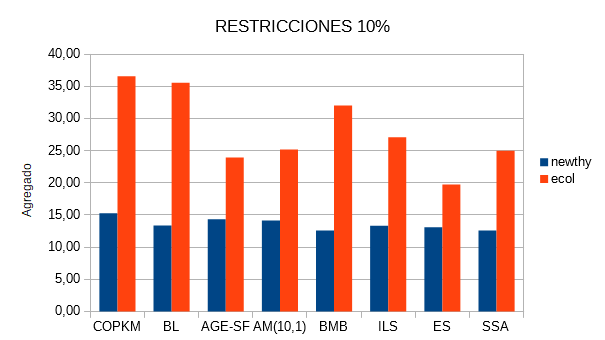
\includegraphics[width=\linewidth]{imagenes/f_10.png}
		\label{fig:boat3}
	\end{figure}

	\begin{figure}[H]
		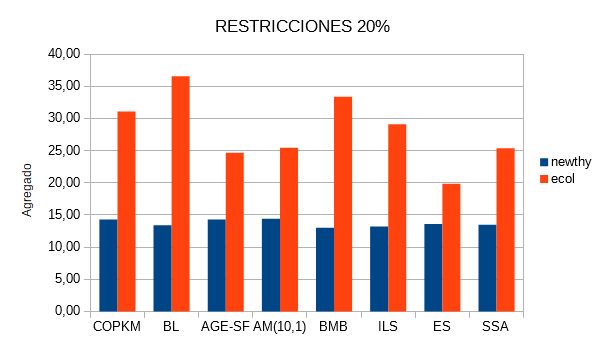
\includegraphics[width=\linewidth]{imagenes/f_20.png}
		\label{fig:boat4}
	\end{figure}
	\newpage
	No obstante, pese a los buenos resultados, encontramos una pega muy importante al uso de SSA. Como vemos en el gráfico de tiempos, el coste computacional de esta técnica es desproporcionadamente superior al del resto de algoritmos usados, encontrando el caso límite en el que estos consumen en torno a 5 segundos para Ecoli, mientras que SSA se demora en torno a 1 hora y 20 minutos. En otros casos no es un problema tan acusado, por ejemplo en Iris tarda unos 20 segundos y en Newthyroid ronda el minuto, pero estamos hablando de conjuntos no demasiado complejos y un número de evaluaciones relativamente bajo, por lo que el algoritmo, a falta de optimización en tiempo, no puede ser considerado como una buena alternativa a cualquiera del resto de algoritmos tan solo por este hecho, no es viable en cuestiones de coste computacional.

	\begin{figure}[H]
		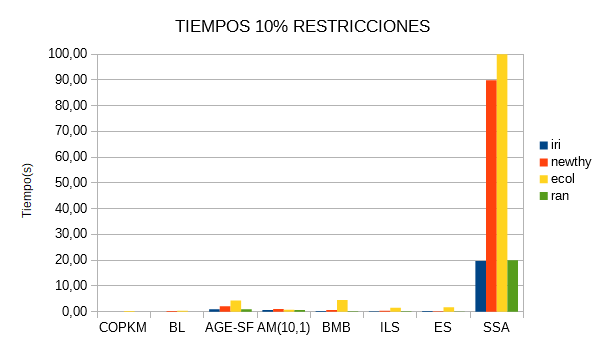
\includegraphics[width=\linewidth]{imagenes/time.png}
		\label{fig:boat5}
	\end{figure}
	
	\subsection{Mejoras durante el desarrollo}
	A continuación se hará una breve descripción de las mejoras realizadas sobre la idea original de la metaheurística.
	\begin{itemize}
		\item Matriz f: Inicialmente los valores f de cada piloto se guardaban en una matriz para ahorrar evaluaciones, sin embargo se llegó a una versión que, eliminando esta matriz, ahorra incluso más evaluaciones.
		\item Optimización en cambio de equipo: El intercambio de pilotos entre equipos tenía el planteamiento de que los mejores vayan a los mejores equipos y viceversa, pero finalmente se ha optado por una solución que debería ser mejor y más simple, y es que cambien aleatoriamente. Con ello se gana en exploración y la implementación de esta parte pasa a ser mucho más sencilla.
		\item Pequeñas optimizaciones: Desde la idea original se han hecho pequeños cambios sin importancia para ahorrar algo de coste.
	\end{itemize}
	\newpage
	\subsection{Posibles futuras mejoras}
	Como última medida se van a comentar posibles mejoras sobre la metaheurística que no se han podido abordar en este proyecto por temas de tiempo.
	\begin{itemize}
		\item BL suave: Siguiendo el ejemplo de los Algoritmos Meméticos es probable que llegue a funcionar mejor usando una BL suave, siendo también menos costosa.
		\item Más optimización en tiempo: Es obvio que si se busca que este algoritmo sea competente es necesario mejorar el tiempo de ejecución en gran medida, lo cual requiere un estudio en conciencia de las partes más costosas y sus posibles mejoras.
		\item Integración de jerarquía en BL: Como pequeña medida, es posible integrar el ajuste de la jerarquía dentro de la modificación de los pilotos, ahorrando evaluaciones en el proceso. No es demasiado relevante ya que no parece estar falta de exploración por ese motivo, pero sí que es posible llevarla a cabo.
	\end{itemize}

	\subsection{Conclusión}
	Podemos concluir por tanto en que se ha llegado a un algoritmo con unos resultados muy competentes, pero que no es viable atendiendo a su tiempo de ejecución. Si se consiguiera optimizar este último sin sacrificar potencia de cálculo sí que tendríamos una metaheurística que podría competir con las ya estudiadas, aunque a pesar de ello, sin un estudio más concienzudo, no se puede saber con certeza si ésto es posible y de donde proviene el gran coste en tiempo de esta técnica.
	
\end{document}